\subsection{Installation}

Installation method of WSL depends on which windows version you are running.

Check your Windows version and build number by pressing\\
\code{Win + R} \ra Entering \code{winver}

\begin{figure}[H]
    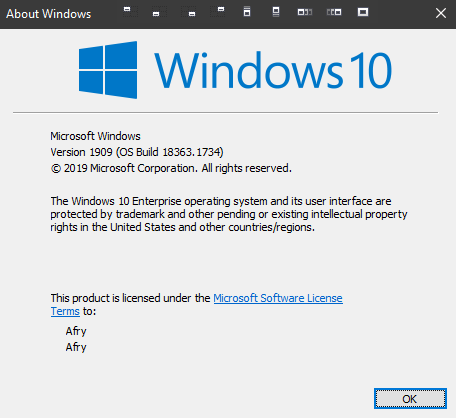
\includegraphics[width=0.55\textwidth]{figures/windows_version.PNG}
\end{figure}

Depending on the version you have, see the below sections.

If you have:
\begin{itemize}
    \item Windows version 2004 and higher, with build 1904 and higher
\end{itemize}
Then you can do the \refsection{sec:automatic_installation}{Automatic installation} section.

If that is not the case, then you must at least have:
\begin{itemize}
    \item Windows version 1903 or higher, with build 18362 or higher
\end{itemize}

If so, then if running the version
\begin{itemize}
    \item 1903, the build number must be 18362.1049 or higher
    \item 1909, the build number must be 18363.1049 or higher
\end{itemize}

If any of those is true for your system, then you can do the \refsection{sec:manual_installation}{Manual installation} section.



\subsubsection{Automatic installation}
\label{sec:automatic_installation}

A simple command in PowerShell:
\code{wsl --install}



\subsubsection{Manual installation}
\label{sec:manual_installation}



\subsubsubsection{Enable Windows Subsystem for Linux}

Open PowerShell as Admin and run:\\
\code{dism.exe /online /enable-feature /featurename:Microsoft-Windows-Subsystem-Linux /all /norestart}



\subsubsubsection{Enable Virtual Machine feature}

Open PowerShell as Admin and run:\\
\code{dism.exe /online /enable-feature /featurename:VirtualMachinePlatform /all /norestart}

Restart your computer.



\subsubsubsection{Download the Linux kernel update package}

Download the latest package through \link{https://wslstorestorage.blob.core.windows.net/wslblob/wsl_update_x64.msi}{this link}.



\subsubsubsection{Set WSL 2 as the default version}

Every new distribution installed should run with the WSL version set as default.

Open PowerShell and run:\\
\code{wsl --set-default-version 2}
